%CP_ant_on_grid

\documentclass[problem]{mcs}

\begin{pcomments}
  \pcomment{from: F01.ps6}
%  \pcomment{}
%  \pcomment{}
\end{pcomments}

\pkeywords{
    state_machine
}

%%%%%%%%%%%%%%%%%%%%%%%%%%%%%%%%%%%%%%%%%%%%%%%%%%%%%%%%%%%%%%%%%%%%%
% Problem starts here
%%%%%%%%%%%%%%%%%%%%%%%%%%%%%%%%%%%%%%%%%%%%%%%%%%%%%%%%%%%%%%%%%%%%%

\begin{problem}

  A hungry ant is placed on an unbounded grid.  Each square of the grid
  either contains a crumb or is empty.  The squares containing crumbs form
  a path in which, except at the ends, every crumb is adjacent to exactly
  two other crumbs.  The ant is placed at one end of the path and on a
  square containing a crumb.  For example, the figure below shows a
  situation in which the ant faces North, and there is a trail of food
  leading approximately Southeast.  The ant has already eaten the crumb
  upon which it was initially placed.

\bigskip
\begin{center}
\includegraphics[width=2in]{figures/ant}
\end{center}
%%\centerline{\resizebox{!}{2.0in}{\includegraphics{figs/ant.eps}}}
\bigskip

The ant can only smell food directly in front of it.  The ant can only
remember a small number of things, and what it remembers after any move
only depends on what it remembered and smelled immediately before the
move.  Based on smell and memory, the ant may choose to move forward one
square, or it may turn right or left.  It eats a crumb when it lands on
it.

% The ant sends a signal whenever it cannot smell food on all 
% four adjacent squares.

The above scenario can be nicely modelled as a state machine in which
each state is a pair consisting of the ``ant's memory'' and
``everything else,'' e.g., information about where things are on the
grid.  Work out the details of such a model state machine; design the
ant-memory part of the state machine so the ant will eat all the
crumbs on \emph{any} finite path at which it starts and then signal
when it is done.  Be sure to clearly describe the possible states,
transitions, and inputs and outputs (if any) in your model.  Briefly
explain why your ant will eat all the crumbs.

\begin{solution}

If all the crumbs are placed as if ``on a string'', then the ant can
pick them all up very easily: If the ant smells no crumb in front of
it, it should turn in some fixed direction (say left), and if it does
smell a crumb, it should go forward and eat it.  Hence the ant can eat
all the crumbs of bread even if it is completely memory-less.
However, we requested that the ant-machine stops and signals {\em
done} when all the bread crumbs are eaten.  If the ant had no memory
then after eating the last crumb it would rotate indefinitely.
Therefore we should embed it with a memory of how many times it
rotated in the same spot in the search of an adjacent bread crumb.  If
the number of turns reaches four, all the bread crumbs are eaten and
the ant can signal {\em done}.  Here is the state machine:
\begin{eqnarray*}
AntMemory &=& \{0,1,2,3,4\}
\\
BoardLocation &=& \naturals \times \naturals
\\
AntDirection &=& \set{N,E,W,S}
\\
Crumbs &\subseteq& BoardLocation
\\
AntLocation &=& BoardLocation
\\
Q &=& AntMemory \times (AntLocation \times AntDirection \times
\mathcal{P}(Crumbs) )
\end{eqnarray*}

The transitions correspond to the three actions \{``go straight'',
``turn left'', ``done''\}.  We will use variables $q=(m,l,d,C)$ to
represent a state $q\in{Q}$ ($m\in{AntMemory}, l\in{AntLocation},
d\in{AntDirection}, C\in{\mathcal{P}(Crumbs)}$).  Let ${\sf Loc}(l,d)$ be a
function taking a location $l\in{AntLocation}$ and
$d\in{AntDirection}$ and returning $l'\in{AntLocation}$ s.t. $l'$ is the
location adjacent to $l$ in direction $d$.  In particular, if the ant
is in location $l$ and goes in direction $d$, it will come to location
$l'={\sf Loc}(l,d)$.  Let ${\sf Next}(d)$ be a function which picks
next direction of an ant which turns left, i.e. ${\sf Next}$ maps N to
W, W to S, S to E, and E to N.

\begin{itemize}
\item
{\sf go straight:}
$(m,l,d,C)\rightarrow(0,{\sf Loc}(l,d),d,C\setminus\{{\sf Loc}(l,d)\})$ if
${\sf Loc}(l,d)\in{C}$.
\item
{\sf turn left:} $(m,l,d,C)\rightarrow(m+1,l,{\sf Next}(d),C)$ if
${\sf Loc}(l,d)\not\in{C}$ and $m\neq{4}$.
\item
{\sf done:} $(m,l,d,C)\rightarrow(m,l,d,C)$ if
${\sf Loc}(l,d)\not\in{C}$ and $m=4$. Furthermore, the ant signals ``done''.
\end{itemize}

\end{solution}

Note that the last transition is a self-loop; the ant signals done for
eternity. One could also add another end state so that the ant signals
done only once.
\end{problem}

%------------------------------------------------
% source: source: spring00 pset4-5
% Based on spring97, handout 28, pset 9 solutions
% topic: marriage problem (simple)
% last used:


%%%%%%%%%%%%%%%%%%%%%%%%%%%%%%%%%%%%%%%%%%%%%%%%%%%%%%%%%%%%%%%%%%%%%
% Problem ends here
%%%%%%%%%%%%%%%%%%%%%%%%%%%%%%%%%%%%%%%%%%%%%%%%%%%%%%%%%%%%%%%%%%%%%

\endinput
